\section{الگوریتم \lr{anti-$k_\mathrm{T}$}}
\label{app:antikt}
الگوریتم \lr{anti-$k_\mathrm{T}$} ذره‌های نهایی هر رویداد را به جت تبدیل می‌کند. ایده آن این است که ذره‌های سخت (با $\pt$ بزرگ) اول با ذره‌های اطرافشان ادغام شوند و جت دور آن‌ها بزرگ شود. برای هر دو شیء $i$ و $j$ (در ابتدا هر ذره یک شیء است) فاصله زیر تعریف می‌شود:
\begin{equation}
d_{ij}=\min\!\left(p_{\mathrm{T},i}^{-2},\,p_{\mathrm{T},j}^{-2}\right)\frac{\Delta R_{ij}^{2}}{R^{2}},\qquad
d_{iB}=p_{\mathrm{T},i}^{-2},
\end{equation}
که در آن $\Delta R_{ij}=\sqrt{\Delta\eta_{ij}^2+\Delta\varphi_{ij}^2}$ فاصله زاویه‌ای دو شیء و $d_{iB}$ فاصله شیء $i$ تا باریکه (\lr{beam}) است. چون $\pt$ با توان منفی در فاصله می‌آید، شیءهای سخت کوچک‌ترین فاصله را دارند. الگوریتم کوچک‌ترین مقدار را از میان همه $d_{ij}$ و $d_{iB}$ پیدا می‌کند. اگر این مقدار یک $d_{ij}$ باشد، دو شیء $i$ و $j$ ادغام می‌شوند (تکانه‌ها جمع می‌شوند و موقعیت جدید با وزن $\pt$ به‌دست می‌آید). اگر یک $d_{iB}$ باشد، شیء $i$ یک جت تمام‌شده است و از فهرست کنار می‌رود. این کار تکرار می‌شود تا هیچ شیئی نماند.

نقش شعاع $R$ را می‌توان مستقیم دید. برای شیء سخت‌تر $i$ داریم $\min(p_{\mathrm{T},i}^{-2},p_{\mathrm{T},j}^{-2})=p_{\mathrm{T},i}^{-2}$، پس $d_{ij}=d_{iB}\,\Delta R_{ij}^2/R^2$. بنابراین $d_{ij}<d_{iB}$ دقیقاً وقتی است که $\Delta R_{ij}<R$ باشد: شیء سخت‌تر فقط با شیءهایی ادغام می‌شود که از $R$ به آن نزدیک‌ترند، و شیءهای دورتر از $R$ هرگز به آن نمی‌پیوندند.

برای دیدن این روند، در شکل~\ref{fig:antikt} پنج ذره با $\pt$ داده‌شده (به \lr{GeV}) آمده است: \lr{A} (۴۰۰)، \lr{B} (۸۰)، \lr{C} (۴۰)، \lr{D} (۲۵) و \lr{E} (۱۵)، با $R=0.8$.
\begin{figure}[!ht]
\centering
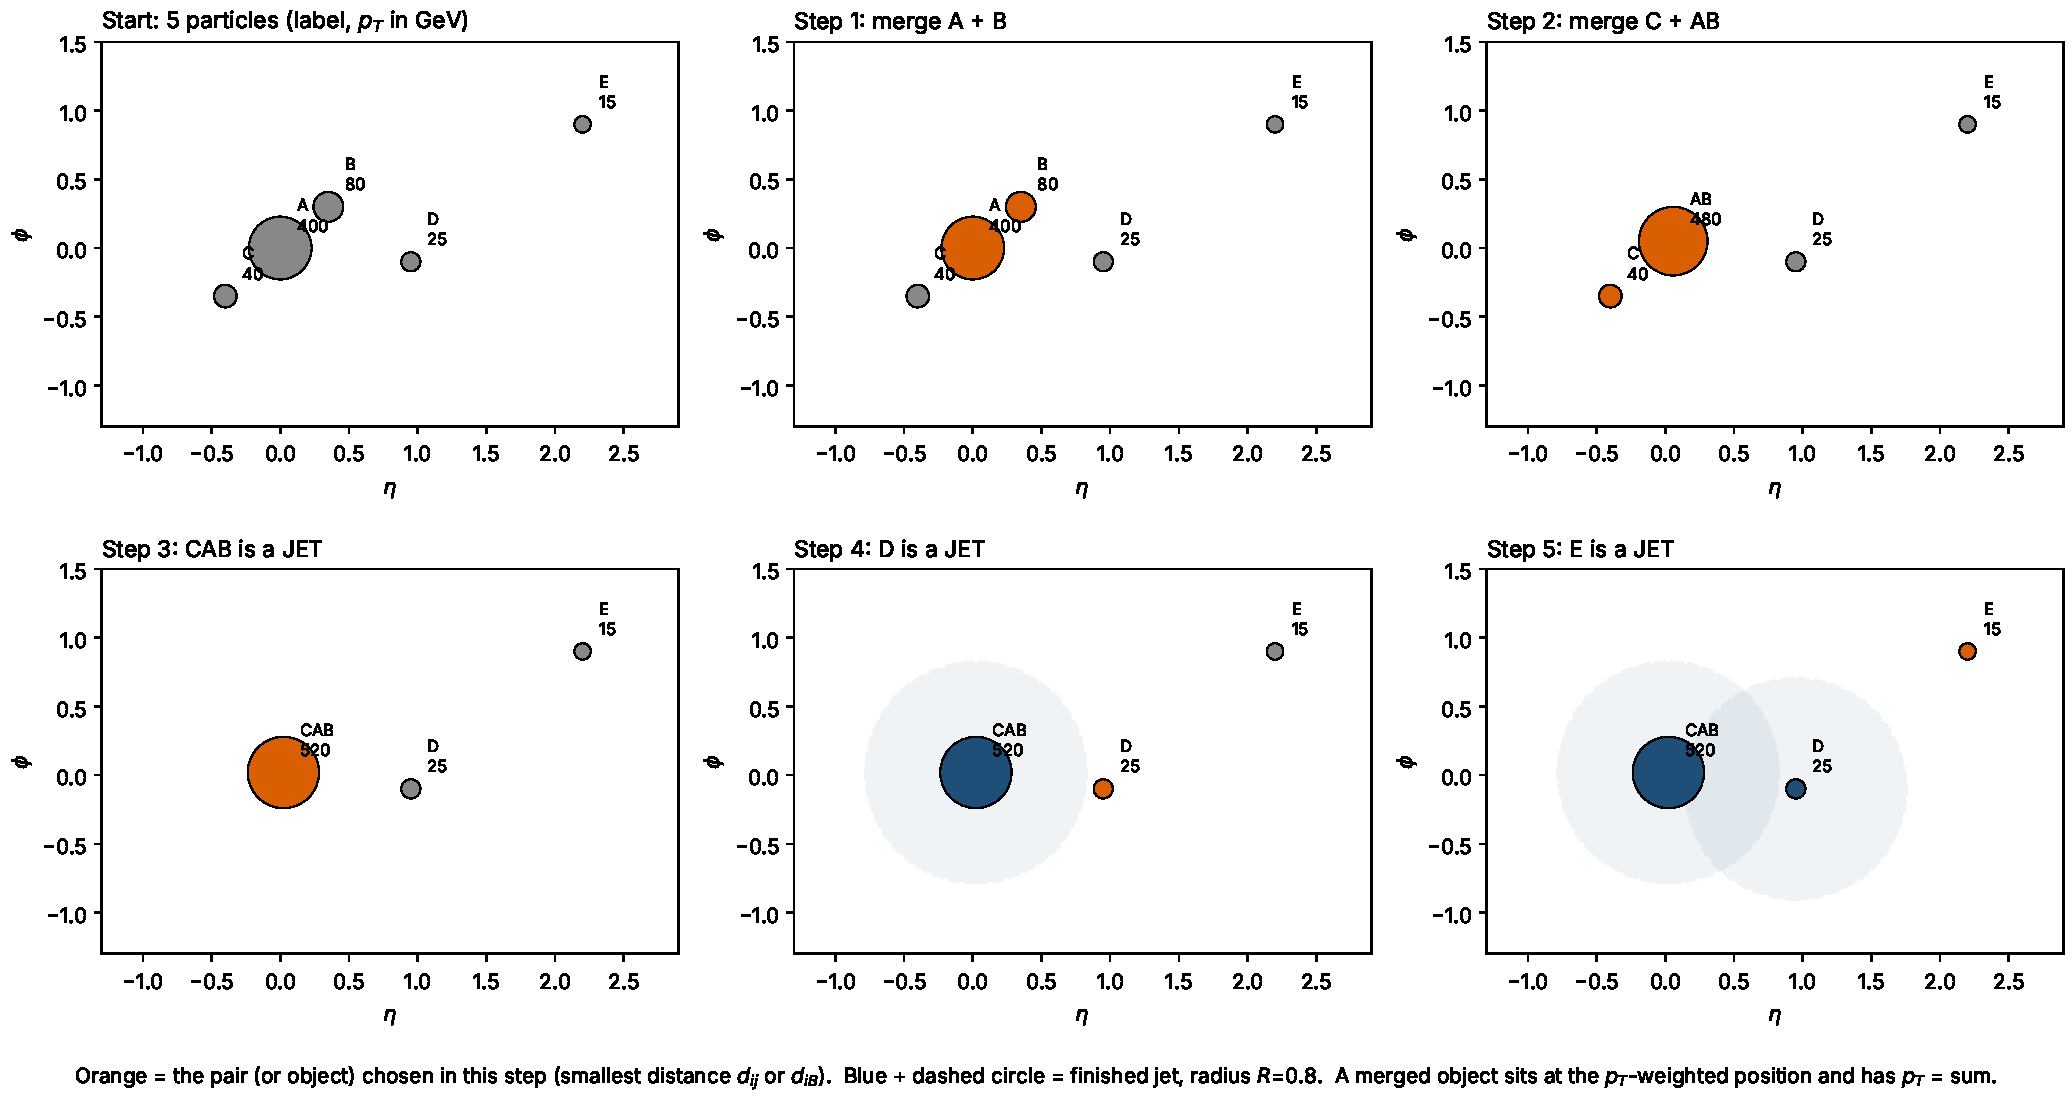
\includegraphics[width=\textwidth]{antikt2.pdf}
\caption{مراحل ساخته شدن جت‌ها با \lr{anti-$k_\mathrm{T}$}. رنگ نارنجی جفت یا شیئی است که در آن مرحله کوچک‌ترین فاصله ($d_{ij}$ یا $d_{iB}$) را دارد. رنگ آبی و دایره خط‌چین (شعاع $R=0.8$) جت تمام‌شده است. شیء ادغام‌شده در موقعیت وزن‌دار با $\pt$ قرار می‌گیرد و $\pt$ آن مجموع دو شیء است.}
\label{fig:antikt}
\end{figure}
ذره سخت \lr{A} ابتدا همسایه‌های خود \lr{B} و بعد \lr{C} را می‌بلعد و شیء \lr{CAB} با $\pt=400+80+40=520$~\lr{GeV} ساخته می‌شود. ذره‌های نرم هرگز اول با هم ادغام نمی‌شوند؛ جت دور هسته سخت رشد می‌کند و ذره‌های نزدیک‌تر زودتر جذب می‌شوند، برای همین جت شکلی گرد دارد. در مرحله بعد باید \lr{CAB} را با \lr{D} مقایسه کنیم که با $\Delta R=0.95$ از آن فاصله دارد. فاصله \lr{CAB} تا باریکه $d_{iB}=1/520^2\approx3.7\times10^{-6}$ است و فاصله تا \lr{D} برابر $d_{ij}=(0.95/0.8)^2/520^2\approx1.41\times3.7\times10^{-6}\approx5.2\times10^{-6}$ است. چون $d_{iB}<d_{ij}$، \lr{CAB} یک جت تمام‌شده می‌شود و \lr{D} به آن نمی‌پیوندد. \lr{D} و \lr{E} نیز با همین استدلال هر کدام یک جت نرم جدا می‌شوند.

جت‌های ساخته‌شده با این الگوریتم ذره مشترک ندارند، چون هر ذره دقیقاً به یک جت تعلق دارد؛ پس تعداد ذرات تشکیل‌دهنده و جرم جت‌های مختلف از هم مستقل‌اند. محور دو جت نیز همیشه بیش از $R$ از هم دور است، چون اگر دو شیء از $R$ نزدیک‌تر بودند ادغام می‌شدند؛ به همین دلیل نمودارهای $\Delta R$ بین دو جت از حدود \lr{0.8} شروع می‌شوند. از نظر هندسی، دایره‌های شعاع $R$ دو جت برای $R<\Delta R<2R$ هم‌پوشانی دارند (در شکل، \lr{CAB} و \lr{D} با $\Delta R=0.95$)، ولی ذره‌های ناحیه مشترک به جت سخت‌تر تعلق دارند و جت نرم‌تر در آن ناحیه بریده می‌شود. در نتیجه هیچ ذره‌ای بین جت منتخب و جت دیگری مشترک نیست و جت سخت یک مخروط تمیز است.

در این پروژه برای $\pt$ در خوشه‌بندی آستانه نگذاشتیم (\lr{inclusive\_jets(0)})، پس هر ذره نرمی که از ذره‌های سخت دورتر از $R$ بود خودش یک جت شد. به همین دلیل بدون آستانه، هر رویداد حدود ۳۳ تا ۳۵ جت دارد (شکل~\ref{fig:s1all}). این‌ها جت واقعی نیستند: جت واقعی آستانه می‌خواهد. تعداد جت‌های باقی‌مانده بعد از هر برش در شکل~\ref{fig:s1njets} (بخش~\ref{sec:cutflow}) آمده است. ما تنها جت‌های با \lr{$\pt>20$~GeV} را ذخیره می‌کنیم.
\widefig{s1_all_njets.pdf}{تعداد جت در هر رویداد بدون آستانه $\pt$.}{fig:s1all}
